\documentclass[en,license=none]{../../../eplsummary}

\usepackage{float}

\graphicspath{{img/}}

\hypertitle{Computer networks}{5}{INGI}{1341}
{Gilles Peiffer}
{Olivier Bonaventure}

\section{Connecting two hosts}

The first step when building a network,
even a worldwide network such as the Internet,
is to connect two hosts together.
In order for two hosts to exchange information,
they need to be linked by some kind of physical medium.
Various types of media have been used for this purpose:
\begin{itemize}
	\item \emph{Electrical cable}.
	Different types of cables are suitable for transmitting information:
	\begin{itemize}
		\item twisted pairs,
		which are used in the telephone network
		and in enterprise networks;
		\item coaxial cables,
		which are used in cable TV networks,
		but not in enterprise networks anymore.
	\end{itemize}
	Some technologies operate over the classical electrical cable.
	\item \emph{Optical fiber}.
	Optical fibers are used in networks
	when the distance between the devices is larger than one kilometer.
	There are two main types of optical fibers:
	\begin{itemize}
		\item multimode, which uses a LED to send signals
		over distances greater than several tens of kilometers;
		\item monomode, which uses a laser to send signals
		over distances of a few kilometers.
	\end{itemize}
	Both types can use repeaters to regenerate the signal
	and send it over another fiber.
	\item \emph{Wireless}.
	With this technology,
	a radio signal is used to encode the exchanged information.
	Modulation techniques are used
	to send information over a wireless channel.
	Some wireless networks use a laser
	that sends light pulses to a detector
	instead of a radio signal.
	These optical techniques allow to create point-to-point links,
	while radio based techniques can be used
	to build networks containing devices
	spread over a small geographical area.
\end{itemize}

\subsection{The physical layer}

The physical media explained previously can be used to exchange information,
once this information has been converted into a suitable electrical signal.
We will focus on the transmission of bits, i.e. either $0$ or $1$.

\begin{mydef}[Bit rate]
	In computer networks, the bit rate of the physical layer
	is always expressed in bits per second.
	This is in contrast with memory specifications
	which are usually expressed in bytes
	(one byte is equal to eight bits).
\end{mydef}

\subsubsection{Time-sequence diagram}

A physical transmission scheme
(interactions between communicating hosts)
can be described by using a \emph{time-sequence diagram}.
By convention, the sender is represented on the left,
and the receiver is on the right.
The middle of the diagram represents the electrical link.
Time flows from top to bottom.
To represent the transmission of a single bit,
three arrows are needed.
\begin{enumerate}
	\item The sender receives a request to transmit one bit of information.
	A \emph{primitive} is used to represent this request,
	sort of like a procedure call.
	The bit being transmitted is the only parameter.
	In the example in \figuref{timeseqdiag},
	the primitive is named \texttt{DATA.request}.
	\item The dashed arrow indicates the signal's propagation time
	between the two hosts.
	Once the signal is received,
	it's interpreted and converted into a bit.
	\item The bit is delivered as a \texttt{DATA.indication} primitive.
\end{enumerate}

\begin{figure}[H]
	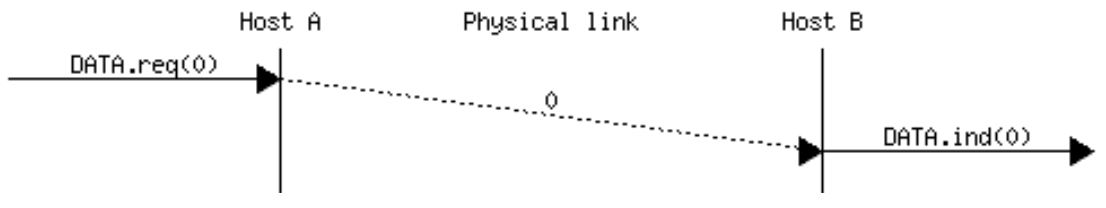
\includegraphics[width=\textwidth]{timeseqdiag.png}
	\caption{A simple time-sequence diagram.}
	\label{fig:timeseqdiag}
\end{figure}

One of the problems of such a transmission scheme
is that electromagnetic interference can switch bits
while they're being transmitted
(i.e. a $0$ bit is sent but a $1$ bit is received).

With the above transmission scheme,
a bit is transmitted by setting the voltage on the electrical cable
to a specific value during some period of time.
One source of errors can be the difference in measured voltage
between the sender and the receiver.
Another reason could be that the two clocks do not operate
at exactly the same frequency.
Small differences in clock frequency imply
that bits can ``disappear'' or ``appear''
during their transmission on an electrical cable
(as in \figuref{lostbitdiag}).

\begin{figure}[H]
	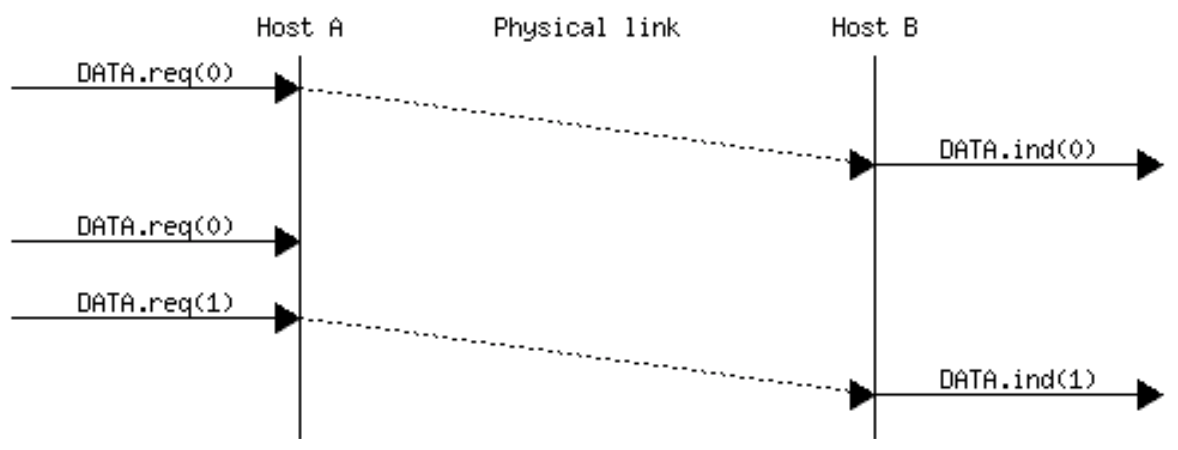
\includegraphics[width=\textwidth]{lostbitdiag.png}
	\caption{Bits can ``disappear'' due to mismatched clock frequencies.}
	\label{fig:lostbitdiag}
\end{figure}

Due to these possible sources of error,
it's important to remember that the physical layer service may
\begin{itemize}
	\item \textbf{change} the value of a bit being transmitted,
	\item \textbf{deliver more (or less)} bits to the receiver
	than the bits sent by the sender.
\end{itemize}

\paragraph{Manchester encoding} Other types of encodings have been defined
to transmit information over an electrical cable.
All physical layers are able to send and receive physical symbols
that represent the values $0$ and $1$.
However, for various reasons that are outside the scope of this chapter,
several physical layers exchange other physical symbols as well.
The Manchester encoding is an encoding scheme
in which time is divided into fixed-length periods.
Each period is divided into two halves
during which different voltage levels (high or low) can be applied.
The four possible combinations make for four possible characters,
as shown in \figuref{manchester_encoding}.

\begin{figure}[H]
	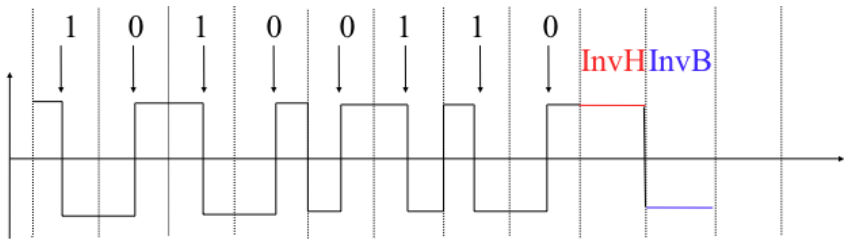
\includegraphics[width=\textwidth]{manchester_encoding.png}
	\caption{Visualisation of the Manchester encoding.
	$0$ and $1$ are regular bits,
	the InvH and InvB symbols can be used as markers
	for the beginning or end of frames.}
	\label{fig:manchester_encoding}
\end{figure}

\subsection{The datalink layer}

The physical layer is the name given
to all the functions related to the physical transmission of information.
It allows two or more entities to exchange bits
if they are connected to the same medium.
Computer networks use different layers,
where each layer provides a service that is built above the underlying layer,
and is close to the needs of the applications.
The datalink layer builds upon the service provided by the physical layer.

% TODO from "The datalink layer"

\end{document}
